\documentclass[preprint]{elsarticle}
% moi them
\usepackage[utf8x]{inputenc}
\usepackage[vietnam]{babel}
\usepackage{algorithm}
\usepackage{algpseudocode}
\renewcommand{\algorithmicrequire}{\textbf{Input:}}
\renewcommand{\algorithmicensure}{\textbf{Output:}}
\usepackage{epsfig}
\usepackage{graphicx}
\usepackage{epstopdf}
\usepackage{booktabs}

\usepackage{lineno,hyperref}
\modulolinenumbers[5]

\journal{Journal of \LaTeX\ Templates}

%%%%%%%%%%%%%%%%%%%%%%%
%% Elsevier bibliography styles
%%%%%%%%%%%%%%%%%%%%%%%
%% To change the style, put a % in front of the second line of the current style and
%% remove the % from the second line of the style you would like to use.
%%%%%%%%%%%%%%%%%%%%%%%

%% Numbered
%\bibliographystyle{model1-num-names}

%% Numbered without titles
%\bibliographystyle{model1a-num-names}

%% Harvard
%\bibliographystyle{model2-names.bst}\biboptions{authoryear}

%% Vancouver numbered
%\usepackage{numcompress}\bibliographystyle{model3-num-names}

%% Vancouver name/year
%\usepackage{numcompress}\bibliographystyle{model4-names}\biboptions{authoryear}

%% APA style
%\bibliographystyle{model5-names}\biboptions{authoryear}

%% AMA style
%\usepackage{numcompress}\bibliographystyle{model6-num-names}

%% `Elsevier LaTeX' style
\bibliographystyle{elsarticle-num}
%%%%%%%%%%%%%%%%%%%%%%%

\begin{document}

\begin{frontmatter}

\title{Eigenclassifier for large scale image classification}
%% Group authors per affiliation:
\author{Elsevier\fnref{myfootnote}}
\address{Radarweg 29, Amsterdam}
\fntext[myfootnote]{Since 1880.}

%% or include affiliations in footnotes:
\author[mymainaddress,mysecondaryaddress]{Elsevier Inc}
\ead[url]{www.elsevier.com}

\author[mysecondaryaddress]{Global Customer Service\corref{mycorrespondingauthor}}
\cortext[mycorrespondingauthor]{Corresponding author}
\ead{support@elsevier.com}

\address[mymainaddress]{1600 John F Kennedy Boulevard, Philadelphia}
\address[mysecondaryaddress]{360 Park Avenue South, New York}

\begin{abstract}
To trade-off between classification accuracy and testing efficiency is one of the challenges in large scale classification. 

In this paper, we propose a new classification approach, called two-step approach, for large scale image classification. Our approach based on factorization matrix approach and training regression functions. The target response matrix obtained by compose matrices which is calculated by regressing on target images... 

Evaluation results on large scale datasets demonstrate the efficiency of proposed approach. Specially, our method achieves comparable accuracy while achieving significantly better testing efficiency with label tree methods.

\end{abstract}

\begin{keyword}
large scale image classification, factorization matrix, label tree
\end{keyword}

\end{frontmatter}

\linenumbers

\section{Introduction}

Classifying an image belongs to one of the C different predefined classes is one of the essential problems in computer vision. 

In the recent years, classifying a large number of  classes  has received increasing attention. There are two main cause, the first is the availability of datasets with hundreds or thousands classes such as Caltech256 \footnote{http://www.vision.caltech.edu/Image\_Datasets/Caltech256/} has 256 object categories and 29,780 images, ILSVRC \footnote{http://www.image-net.org/challenges/LSVRC/} has 1K categories and 1.2 million images, 
SUN Dataset \footnote{http://groups.csail.mit.edu/vision/SUN/} has 908 scene categories and 131,067 images,
ImageNet  \footnote{http://www.image-net.org/} has 22K synsets and 14 million images.

The second is increasing a number of images in photo-sharing websites such as Flickr, Facebook, Instagram, ... 
It requires the scalable methods that is both accuracy and efficiency when there are a large number of classes and samples.

One of the significant challenges in large scale classification that is how to trade-off between accuracy and test time. 

The methods based on binary classifiers, for example one-vs-all strategy, show good classification accuracy. However, due to all classifies have to be evaluated at run time for every image, the time complexity scale linearly up the number of classes. They could become impractical when there are a large number of classes and target images.

Recently, the tree-based methods using hierarchical structure to organize set of classes into label tree has been show to good trade-off accuracy and test time. In theory, the time complexity reduce sublinearly with the number of classes, $logC$-times evaluation of classifiers for $C$ classes. Although, the different small set of classifiers should be evaluated for each target image, $C$ (binary tree case) or $\frac{Q}{Q-1}C$ (Q-way tree case) should be prepared. Moreover, to make prediction given a target image, we traverse the tree from the root until we reach a leaf node. So it is taken the time to select the branch and change classifiers. They could be slow in practice.

In this paper, we propose a novel method for multi-class large scale classification without using hierarchical structure. By factorizing response matrix $R_{N \times C}$, which is obtained by applying $C$ classifiers using one-vs-all strategy to $N$ validated images,  into matrix $U_{N \times K}$ and matrix $V_{K \times C}$, namely, $R=UV$. And then training regression functions $g_k$ with given $U$. In classification, we calculate matrix $U_{M \times K}^{test}$ for $M$ test images using regression functions $g_k$ and obtain response matrix $R_{M \times K}^{test}$, namely, $R^{test}= U^{test}V$. To archive a good trade-off between classification accuracy and test time. bằng cách chọn giá trị k thích hợp. Specially, if the value of k is equal with number classifies used for evaluation in label tree, our method is not only comparable about accuracy but also  better efficiency about test time.


\section{Related work}

\subsection{Classification}
Về cơ bản có hai cách tiếp cập để giải quyết, hướng tiếp cận dựa trên các bộ phân lớp nhị phân và hướng tiếp cận dựa trên cây phân cấp các lớp.

Các phương pháp trong hướng tiếp cận 1 sử dụng kết quả từ các bộ phân lớp nhị phân để xác định kết quả phân lớp cho ảnh. Ưu điểm của các phương pháp này là dễ lập trình, tuy nhiên, khi thực hiện phân lớp cho một ảnh ta phải thực hiện phân lớp qua tất cả các bộ phân lớp để xác định kết quả phân lớp. Trong trường hợp large scale, khi mà số lượng lớp từ hàng trăm, đến hàng chục ngàn và số lượng ảnh từ hàng ngàn đến hàng triệu ảnh, thì việc thực hiện phân lớp như thế sẽ trở nên không khả thi.

Để giảm chi phí thực hiện phân lớp, các phương pháp theo hướng tiếp cận thứ hai tổ chức các lớp theo một cấu trúc cây phân cấp, các node lá trong cây tương ứng với các lớp, các node trung gian có tác dụng xác định xem ảnh cần phân lớp sẽ thuộc nhánh nào trong các nhánh con của nó. Quá trình phân lớp được thực hiện từ node gốc, duyệt qua các node trung gian cho đến khi gặp node lá, ảnh sẽ được phân vào lớp tương ứng với node lá. Mặc dù chi phí thực hiện phân lớp cho một ảnh theo hướng tiếp cận này giảm còn O(log n). 

\subsection{SVD}

\section{Our method}
\subsection{Overview of the method}

Giả sử một tập các ảnh tset cần được phân lớp đã load vào trong bộ nhớ. 
- Đối với pp label tree, chúng ta phải phân lớp cho từng ảnh. 
+ Vì thế nó mất chi phí cho phép gán các phần tử.
+ Chi phí để phân lớp tại một node, tối thiểu là Q classifier in balanced Q-way tree case.
+ Chi phí để lựa chọn nhánh con tiếp theo.
+ Chi phí xác định kết quả ( vì một ảnh có thể duyệt nhiều nhánh nên sẽ có nhiều kết quả )
-Đối với pp của của chúng tôi
+ Chi phí regression cho một tập các ảnh
+ Chi phí nhân ma trận để tạo ra ma trận kết quả
+ Chi phí đánh xác định kết quả 
 
 
 Các pp phân lớp hiện nay hầu như đềudựa trên giá trị response của các classifers để xác định kết quả phân lớp cho 1 ảnh. 



\begin{figure*}
\begin{center}
\fbox{\rule{0pt}{2in} \rule{.9\linewidth}{0pt}}
\end{center}
   \caption{Example of a short caption, which should be centered.}
\label{fig:short}
\end{figure*}

\subsection{Two-step approach}
We factorize $N$ by $C$ response matrix $R$ into $N$ by $L$ matrix $P$ and $L$ by $C$ matrix $Q$, namely, $R=PQ$. One way to do this is to use singular value decomposition (SVD for short):
\begin{equation}
R = U \Sigma V^T \label{eq:svds}
\end{equation}

We can approximate $R$ in MSE sense by using singular vectors corresponding to $L$-largest singular values. This implies $f'$ to be linear combination of $g_k$. In training, based on the obtained $U=[u_1,u_2,...,u_L]$, we train functions $g_k$ which well approximates $u_k$, namely, $g_k(v_i) \approx u_{(i,k)}$. We can use regression to train $g_k$ given $U$. In classification, we calculate $U$ for the target data using $g_k$,
\\
\\

\begin{algorithm}
  	\caption{training}\label{alg_training}
  	\begin{algorithmic}
	\State 
	\begin{enumerate}[Step 1.]
	\item Obtain $R$ from training label, or first train $C$ classifiers using one-vs-all strategy, and obtain responses of $C$ classifiers for $N$ images.
 
	\item Decompose $R$ via singular value decomposition, namely, $R = U \Sigma V^T$ and obtain $U$, $\Sigma$ and $V$. Keep only $L$ largest singular values and corresponding singular vectors.

	\item For each $u_k, k=1,...,L$ where $U=[u_1,u_2,...,u_L]$, train regression function $g_k(v)$ (SVR can be used).
\end{enumerate}
	\end{algorithmic}
\end{algorithm}

\begin{algorithm}
  	\caption{classification}\label{alg_classification}
  	\begin{algorithmic}
	\State 
	\begin{enumerate}[Step 1.]
	\item Given feature vectors of target images, obtain responses of regression function $g_k$ and obtain $U_{test}$.

\item Calculate estimated response by $R_{test} = U_{test} \ Sigma V^T$ using $\Sigma$ and $V$ obtained during training.

\item Output classification results (either as multi-classification using max operator or as multiple binary classification using thresholding) from $R_{test}$
\end{enumerate}
	\end{algorithmic}
\end{algorithm}



{\bf pros} Linear factorization such as SVD is fast and preferable for theoretical analysis. SVD with SVR (Support Vector Regression) achieves reasonable performance.\\\\
{\bf issues} It is unknown what kind of factorization is better. It is unknown what kind of regression is better.\\\\
{\bf cons} Due two-stage approach, approximation error may occur in each stage.

Nếu các hàm gk là linear thì chúng ta tính trực tiếp $Utest = S^TW$ ????


\section{Experiments}

Usually, experiments are conducted to evaluate how the proposed method works 
– Experimental setup 
– Test sets
– Procedure
– Arrangement of resulting data (graph and table]
– Comprehensive comparison with existing methods 
[fairness] 

\subsection{Datasets}
To facilitate experimentation and comparison of results, we evaluate our method on several datatsets that are often used in experiments for large scale image classification, including Caltech256, SUN397 and ImageNet1K.

\textbf{Caltech256} The Caltech256 is a standard multiclass dataset with 256 classes, 29,780 images and at least 80 images per class. It is used for evaluation in tree and flat based methods.

\textbf{SUN 397} The SUN397 consist of 108,754 images in 397 classes which is sampled from the SUN Dataset has 908 scene categories. 

\textbf{ImageNet1K} The ImageNet1K or ILSVRC2010 is a subset of ImageNet. It consist of 1,2M images in 1K classes for training (at least 668 images per class), 50K images for validation (50 images per class) and 150K images for testing (150 images per class).  

\subsection{Experimental setup}
For Caltech256 and SUN397, we split the original dataset to three disjoint dataset by 50\% for training, 25\% for validation and the rest 25\% for testing.

For ImageNet1K, due to lack of memory, we randomly pick 300 images of each class for training,  và sử dụng cùng tập validation và testing của dataset.

Due to we is only interesting in the performance of method and to be able to comparable with others, the feature vectors is represented in the same fashion as[xxx]. Each image is extracted dense SIFT features using VLFeat toolbox. These features were pooled using two level spatial pyramid ($1 \times 1$ and $2 \times 2$ with LLC encoding strategy. With the size of code book is 10,000 visual words, the dimension of feature vector is 50,000.

LIBLINEAR library is used to training both one-vs-all classifiers and regression functions with default valued parameters.

\subsection{Evaluation Measurement}
The classification performance is often measured using accuracy and test speedup. However, in practice we found that đề phản ánh hiệu quả của các phương pháp khi thực phân lớp, thì thời gian thưc để thực hiện phân lớp cần được xét đến. 

\subsubsection{Global accuracy}
 The classification accuracy ($Acc$) is a popular measurement to evaluate accuracy rate. It is defined following:
\begin{equation}
Acc = \frac{1}{m} \sum_{i=1}^{m}  1(\hat{y}_i=y_i)
\end{equation}
where, $m$ is a number of target images and $1(\hat{y}_i=y_i)$ is a indicator function, $1(\hat{y}_i=y_i)=1$ if predicted class $\hat{y}_i$ is the same with assigned class $y_i$ of image $x_i$, otherwise, $1(\hat{y}_i=y_i)=0$

\subsubsection{Test speedup} 
The test speedup ($S_{te}$) is the one-vs-all test cost divided by the label tree test cost. Test costs are measured as average number of vector operations performed for classifying a testing example.
   

Độ đo Test speedup  được dùng để so sánh tính hiệu quả của pp dùng cây với các phương pháp trong hướng tiếp cận phẳng, do đó nếu phương pháp trong tiếp cận phẳng là OVA thì phương pháp phân $Q$ lớp tại node $r$ sẽ là OVA. Ta cần lưu ý là số mẫu để huấn luyện trong hai trường hợp này khác nhau, trong phương pháp OVA của hướng tiếp cận phẳng thì số ảnh mẩu được sử dụng là tất các các ảnh từ $n$ lớp trong khi phương pháp OVA tại node $r$ chỉ dùng tất cả các ảnh của $|l(r)|$ lớp thuộc vào node này, giá trị $|l(r)| \le  n$. Do đó, sử dụng mô hình SVM với nhân tuyến tính (linear kernel) thì chi phí ước lượng giá trị phân lớp trên ảnh $x$ trong hai trường hợp này như nhau, nhưng nếu sử dụng mô hình SVM với nhân phi tuyến (nonlinear kernel) thì chi phí ước lượng giá trị phân lớp sẽ phụ thuộc vào số lượng SVs trong từng mô hình. Để khắc phục vấn đề này, ta có thể thực hiện chuyển đổi đặc trưng theo hàm nhân phi tuyến rồi áp dụng mô hình SVM với nhân tuyến tính. Vì thế để đánh giá tính hiệu quả của các phương pháp phân lớp dựa trên cây ta thường sử dụng tuyến tính để thực hiện phân lớp tại các node \cite{Gao.ICCV2011}. 


\subsubsection{Computation time}

Thời gian tính toán  là một yếu tố cần quan tâm trong thực tế khi thực hiện phân lớp một tập m ảnh với số lượng lớn.

Độ đo Ste chỉ quan tâm đến số phép dot product được sử dụng khi thực hiện phân lớp. Trong label tree, mặc dù chỉ một số lượng nhỏ các lớp được sử dụng để phân lớp 1 ảnh nhưng không phải tất cả các lớp này được evaluated cùng lúc, chẳng hạn với balanced tree T10,3, để phân lớp cho 1 ảnh thì tổng số classifier được dùng là 30, nhưng tại mỗi node trên đường đi từ node root đến node lá thì chỉ có 10 classifier được evaluated. 

Ngoài ra, ta cần phải có chi phí ước lượng to decide which branch to follow. .....

\section{Results and Discussion}
Re: Elsevier Table Format
\begin{tabular}{ccc}
  \toprule
  1 & 2 & 3 \\
  \midrule
  4 & 5 & 6 \\
  7 & 8 & 9 \\
  1 & 2 & 3 \\
\end{tabular} 

\subsection{Accuracy comparison}

\begin{table}
\caption{ ... text above table ... }
\begin{center}
\begin{tabular}{|l|c|c|c|c|c|c|c|c|c|c|}
\hline
Method &  \multicolumn{2}{ |c| }{Flat}	&	\multicolumn{2}{ |c| }{T32,2} 	&	\multicolumn{2}{ |c| }{T10,3} &		\multicolumn{2}{ |c| }{T6,4} \\
\hline\hline

							&	Acc\%	& Ste &	Acc\% &	Ste	&	Acc\%	& Ste &	Acc\%	& Ste  \\
\hline
NaiveLabel Tree (Bengio) 	&   &	& 7.3	& 15.79	& 5.18	& 33.33	& 4.66	& 42.51  \\ 
\hline
F\&B Tree (Deng)			&   &	& 11.9	& 10.3	& 8.92	& 18.20	& 5.62	& 31.3 \\ 
\hline
ProbTree (Liu)				&   & 	& 21.38	& 10.42	& 20.54	& 17.85	& 17.2	& 31.25  \\ 
\hline
Our method			&   & 	& 20.31	& 10.42	& 16.96	& 17.86	& 11.67	& 31.25  \\ 
\hline
LIBLINEAR (ProbTree)		& 24.84	& 1		& \multicolumn{6}{ |c| }{}	\\	
\hline
LIBLINEAR (Our)				& 26.01	& 1		& \multicolumn{6}{ |c| }{}	\\ 
\hline
\end{tabular}
\end{center}

\end{table}

--------------------------

\begin{table}
\caption{ ... text above table ... }
\begin{center}
\begin{tabular}{|l|c|c|c|c|c|c|c|c|}
\hline
Method & \multicolumn{2}{ |c| }{Flat}	&	\multicolumn{2}{ |c| }{T20,2} &	\multicolumn{2}{ |c| }{T10,3} &	\multicolumn{2}{ |c| }{T5,4} \\
\hline\hline

&	Acc\%	& Ste &	Acc\% &	Ste	&	Acc\%	& Ste &	Acc\%	& Ste \\
\hline
NaiveLabel Tree (Bengio) & &	& 24.89	& 9.98	& 20.97	& 15.81	& 17.73	& 20.34 \\
\hline
Our method	& & & 29.09	& 9.93	& 24.04	& 15.88	& 20.19	& 20.89 \\ 
\hline
LIBLINEAR (Our)	& 43.33	& 1	& \multicolumn{6}{ |c| }{}	\\ 
\hline
\end{tabular}
\end{center}
\end{table}




Code Tabe cua Caltech 256
\begin{table}
\caption{Results. Ours is better.}
\begin{center}
\begin{tabular}{|l|c|c|c|c|c|c|c|c|}
\hline
Method & \multicolumn{2}{ |c| }{Flat}	&	\multicolumn{2}{ |c| }{T16,2} &	\multicolumn{2}{ |c| }{T7,3} &	\multicolumn{2}{ |c| }{T4,4} \\
\hline\hline

&	Acc\%	& Ste &	Acc\% &	Ste	&	Acc\%	& Ste &	Acc\%	& Ste \\
\hline
NaiveLabel Tree (Bengio) & &	& 30.99	& 8	& 27.34	& 12.67	& 26.01	& 16 \\
\hline
Our method	& & & 33.38	& 8	&25.45	& 12.8	&22.08	& 16\\
\hline
LIBLINEAR (Our)	& 50.95	& 1	& \multicolumn{6}{ |c| }{}	\\ 
\hline
\end{tabular}
\end{center}

\end{table}
\subsection{Computation time}

\subsection{Trade-off the Accuracy - Efficiency}

\begin{figure}
\vspace{30mm} % height of figure
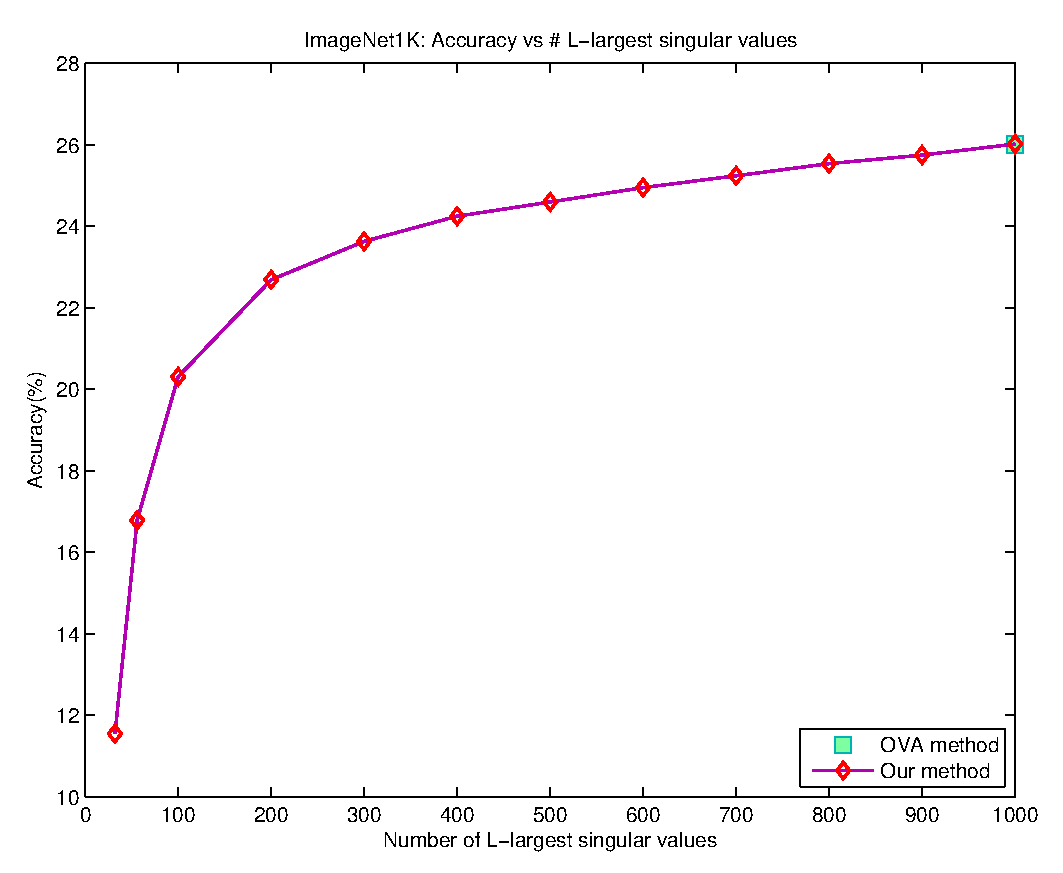
\includegraphics[width=0.8\linewidth]{Figure_ILSVRC_Acc_2step.eps}
\caption{ ... text below figure ... }
\end{figure}


\begin{figure}
\vspace{30mm} % height of figure
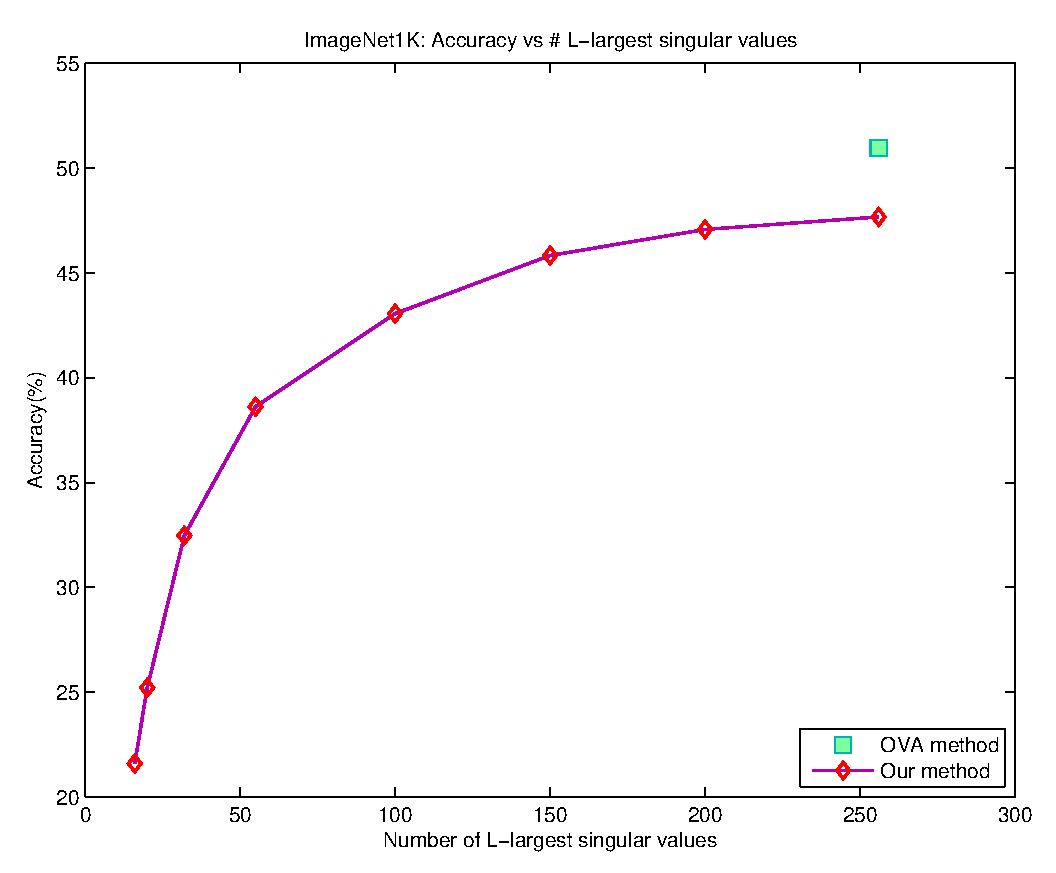
\psfig{file=Figure_Caltech256_Acc_2step.eps, scale=0.8, height=3in}.
\caption{ ... text below figure ... }
\end{figure}

\section{Conclusion}

+Good conclusion enhances reviewer's clear understanding of the work 
+Should not be a copy of Abstract 
+May contain: 
– Contribution to the particular area 
– Novelty and practical significance 
– Limitation and/or weakness of the work to avoid
reviewers’ “attack” 
– Future works for further improvement 



\section{Bibliography styles}

There are various bibliography styles available. You can select the style of your choice in the preamble of this document. These styles are Elsevier styles based on standard styles like Harvard and Vancouver. Please use Bib\TeX\ to generate your bibliography and include DOIs whenever available.

Here are two sample references: \cite{Feynman1963118,Dirac1953888}.

\section*{References}

\bibliography{mybibfile}

\end{document}